\documentclass[11pt]{article}
\usepackage{CJKutf8}
\usepackage{geometry}
\geometry{margin=1in}
\usepackage{amsmath,amssymb,amsthm}
\usepackage{microtype}
\usepackage{booktabs}
\usepackage{tikz-cd}
\usepackage{tikz}
\usetikzlibrary{positioning, decorations.pathreplacing}
\usepackage[colorlinks=true,
  linkcolor=blue!60!black,
  citecolor=teal!60!black,
  urlcolor=magenta!70!black]{hyperref}

% theorem environments
\theoremstyle{definition}
\newtheorem{definition}{Definition}[section]
\newtheorem{remark}[definition]{Remark}
\newtheorem{example}[definition]{Example}
\theoremstyle{plain}
\newtheorem{theorem}[definition]{Theorem}
\newtheorem{corollary}[definition]{Corollary}
\newtheorem{lemma}[definition]{Lemma}
\newtheorem{proposition}[definition]{Proposition}

% macros
\newcommand{\Z}{\mathbb{Z}}
\newcommand{\N}{\mathbb{N}}
\newcommand{\cjk}[1]{\begin{CJK}{UTF8}{gbsn}#1\end{CJK}}

\title{\textbf{Fiber Product Structure in Cyclic Calendar Systems}\\[0.3em]
\large With a Theorem on Additive Distance Optimality}
\author{Alejandro Radisic}
\date{\today}

\begin{document}
\maketitle

\begin{abstract}
We study the algebraic structure of cyclic calendar systems and the problem of optimal symmetric pairings on finite products of cyclic groups.

\textbf{Structure.} The Mesoamerican Calendar Round and the Chinese Sexagenary Cycle both decompose naturally as fiber products of their constituent cycles: $\Z_{18980} \cong \Z_{260} \times_{\Z_5} \Z_{365}$ and $\Z_{60} \cong \Z_{10} \times_{\Z_2} \Z_{12}$. The shared components ($\Z_5$ and $\Z_2$ respectively) constrain the symmetry group and correspond to culturally recognized features---a shared day-count position and yin/yang parity. These fiber product structures arise independently in unconnected civilizations.

\textbf{Optimality.} For any finite product of cyclic groups $\Z_{n_1} \times \cdots \times \Z_{n_k}$ equipped with the \emph{product metric} (sum of circular distances on each factor), the minimum total cost among orbit-respecting matchings is achieved by simple coordinate reflections alone. The proof reduces to a single arithmetic inequality via cost additivity. This theorem applies to the CRT decomposition of the calendar systems above but \emph{not} to the native circular metric on $\Z_n$, since the Chinese Remainder Theorem is a group isomorphism, not an isometry. The theorem fails on the Boolean hypercube $\{0,1\}^n$ under Hamming distance, where composites can outperform simple operations.

All main results are kernel-checked in Lean~4; the Calendar Round proof ($n = 18980$) is fully structural.
\end{abstract}

\section{Introduction}

Many cultures organize time using cyclic calendar systems: repeating sequences of days, years, or ritual periods. When such a system combines multiple cycles of different lengths, the resulting structure is richer than a simple modular count. We identify a recurring algebraic pattern---fiber product decomposition---in two historically independent calendar traditions, and study an optimization problem on the product structure that arises from this decomposition.

\paragraph{Structural observation.} Calendar systems that combine two cycles of lengths $m$ and $n$ with $\gcd(m, n) > 1$ naturally decompose as fiber products $\Z_m \times_{\Z_d} \Z_n$, where $d = \gcd(m, n)$. The shared $\Z_d$ component constrains which pairs of cycle positions can co-occur, reducing the symmetry group and creating a ``locked'' factor. We show this pattern appears in both the Mesoamerican Calendar Round ($\Z_{260} \times_{\Z_5} \Z_{365}$, with shared $\Z_5$) and the Chinese Sexagenary Cycle ($\Z_{10} \times_{\Z_2} \Z_{12}$, with shared $\Z_2$ corresponding to yin/yang parity).

\paragraph{The optimization problem.} Via the Chinese Remainder Theorem, the non-locked factors of such systems form a product of cyclic groups $\Z_{n_1} \times \cdots \times \Z_{n_k}$. On this product, we consider the \emph{product metric}: the sum of circular distances on each factor. This is \emph{not} the same as the native circular distance on $\Z_n$ (the CRT is a group isomorphism, not an isometry). Under this product metric, we ask: among orbit-respecting matchings via coordinate reflections, can composites beat simple reflections?

\paragraph{Main finding.} For any product of cyclic groups with the product metric, the answer is \emph{no}: simple reflections always suffice. This contrasts sharply with the Boolean hypercube under Hamming distance, where composites can strictly outperform simple operations.

\paragraph{Scope.} All cultural references (calendar systems, divination traditions) serve as mathematically concrete examples. No historical or anthropological claims are made unless explicitly stated. The structural observations (fiber products, shared components) are independent of the optimality theorem.

\paragraph{Context.} This paper extends prior work on the Boolean hypercube~\cite{radisic2026iching}, which established that the King Wen sequence of the I Ching encodes an optimal matching under a different symmetry structure. Here we identify the precise criterion---generator locality---that distinguishes systems where simple reflections suffice from those requiring composite operations.

\medskip

We now formalize this setting. Let $X = \Z_{n_1} \times \cdots \times \Z_{n_k}$ be a finite product of cyclic groups, equipped with the \emph{product metric} (also called the $\ell^1$ or Manhattan distance on the product):
\[
d(x, y) = \sum_{i=1}^k d_{n_i}(x_i, y_i)
\]
where $d_n(a, b) = \min(|a - b|, n - |a - b|)$ is the circular distance on $\Z_n$. Concretely, $d_n(a,b)$ measures the shorter arc length between $a$ and $b$ on a circle of $n$ equally spaced points.

\begin{remark}[Product Metric vs.\ Native Circular Metric]\label{rem:metric}
When $\Z_n \cong \Z_{n_1} \times \cdots \times \Z_{n_k}$ via the Chinese Remainder Theorem, the product metric $d$ on the right-hand side is \emph{not} the same as the circular distance $d_n$ on $\Z_n$ itself. The CRT is a group isomorphism but not an isometry. For example, $d_{60}(1, 2) = 1$ but $d_5(1, 2) + d_4(1, 2) + d_3(1, 2) = 3$. All optimality results in this paper concern the product metric. The structural results (fiber product decompositions, shared components, symmetry reduction) are metric-independent.
\end{remark}

The group $G = \Z_2^k$ acts on $X$ by coordinate negation: generator $g_i$ sends $(x_1, \ldots, x_i, \ldots, x_k)$ to $(x_1, \ldots, n_i - x_i, \ldots, x_k)$. Composite elements negate multiple coordinates simultaneously.

\begin{definition}[Orbit-Respecting Matching]\label{def:matching}
Let $G$ act on a finite set $X$. An \emph{orbit-respecting matching} is an involution $\phi: X \to X$ such that $\phi(x) \in G \cdot x$ for all $x \in X$ (i.e., each element is paired with another element in its orbit). The \emph{total cost} is $(1/2) \sum_{x \in X} d(x, \phi(x))$. The factor of $1/2$ corrects for double-counting each pair $\{x, \phi(x)\}$.
\end{definition}

\begin{figure}[ht]
\centering
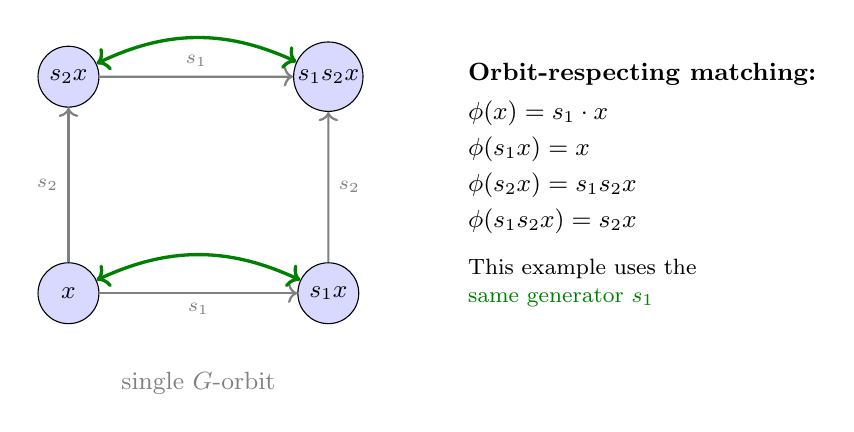
\begin{tikzpicture}[scale=1.1,
    vertex/.style={circle, draw, fill=blue!15, minimum size=22pt, inner sep=1pt, font=\small},
    action/.style={->, gray, thick},
    matching/.style={<->, green!50!black, very thick, bend left=25}
  ]
  % Orbit vertices (square arrangement)
  \node[vertex] (x) at (0, 0) {$x$};
  \node[vertex] (s1x) at (3, 0) {$s_1 x$};
  \node[vertex] (s2x) at (0, 2.5) {$s_2 x$};
  \node[vertex] (s1s2x) at (3, 2.5) {$s_1 s_2 x$};

  % Group action edges (gray, showing orbit structure)
  \draw[action] (x) -- node[below, font=\scriptsize] {$s_1$} (s1x);
  \draw[action] (s2x) -- node[above, font=\scriptsize] {$s_1$} (s1s2x);
  \draw[action] (x) -- node[left, font=\scriptsize] {$s_2$} (s2x);
  \draw[action] (s1x) -- node[right, font=\scriptsize] {$s_2$} (s1s2x);

  % Equivariant matching (via s_1) - curved green arrows
  \draw[matching] (x) to (s1x);
  \draw[matching] (s2x) to (s1s2x);

  % Labels
  \node[anchor=north, font=\small, gray] at (1.5, -0.8) {single $G$-orbit};

  % Right side: explanation
  \node[anchor=west, align=left, font=\small] at (4.5, 1.25) {%
    \textbf{Orbit-respecting matching:}\\[3pt]
    $\phi(x) = s_1 \cdot x$\\[2pt]
    $\phi(s_1 x) = x$\\[2pt]
    $\phi(s_2 x) = s_1 s_2 x$\\[2pt]
    $\phi(s_1 s_2 x) = s_2 x$\\[6pt]
    {\footnotesize This example uses the}\\[-1pt]
    {\footnotesize \textcolor{green!50!black}{same generator $s_1$}}
  };
\end{tikzpicture}
\caption{Orbit-respecting matching on a $\Z_2 \times \Z_2$ orbit. Gray arrows show the group action; green arrows show an orbit-respecting matching via $s_1$. Each element is paired with another element \emph{in the same orbit} via some $g \in G$. The involution condition ($\phi^2 = \mathrm{id}$) ensures symmetric pairing.}
\label{fig:orbit}
\end{figure}

\begin{remark}[Why Orbit-Respecting?]
Three motivations for the orbit-respecting constraint:
\begin{enumerate}
    \item \textbf{Mathematical naturality.} Without this constraint, the optimal matching is trivial: pair each $x$ with its nearest neighbor. This degenerates to a bipartite matching problem with no algebraic structure. Requiring $\phi(x) \in G \cdot x$ restricts to matchings that ``respect the symmetry,'' yielding a richer optimization landscape.
    \item \textbf{Structural content.} The involution condition $\phi^2 = \mathrm{id}$ ensures $\phi$ partitions $X$ into pairs (a perfect matching). The orbit condition $\phi(x) \in G \cdot x$ keeps each pair within a single orbit. Together, these ensure the matching respects the orbit structure of the group action.
    \item \textbf{Implicit in applications.} Pairing systems in calendrical and divinatory traditions often exhibit reflection symmetry: ``opposite'' days, complementary symbols, yin/yang duality. The orbit-respecting condition formalizes this implicit structure.
\end{enumerate}
\end{remark}

\begin{definition}[Simple-Generator Matching]
An orbit-respecting matching $\phi$ is \emph{simple} if for each $x$, we have $\phi(x) = s \cdot x$ for some generator $s \in S$ (i.e., $s$ reflects exactly one coordinate).
\end{definition}

\begin{example}[Sexagenary Cycle under Product Metric]\label{ex:sex}
Consider the Sexagenary Cycle $\Z_{60} \cong \Z_5 \times \Z_{12}$ (via CRT). For year $y = 7$, we have $(y \bmod 5, y \bmod 12) = (2, 7)$. Under the \emph{product metric} $d = d_5 + d_{12}$, the simple reflections are:
\begin{itemize}
    \item $s_1$: negate $\Z_5$ component $\to (5-2, 7) = (3, 7) \to$ year $43$, with product cost $d_5(2, 3) = 1$
    \item $s_2$: negate $\Z_{12}$ component $\to (2, 12-7) = (2, 5) \to$ year $17$, with product cost $d_{12}(7, 5) = 2$
\end{itemize}
The composite $s_1 s_2$ yields $(3, 5) \to$ year $53$, with product cost $1 + 2 = 3$. The best simple reflection ($s_1$, cost 1) beats the composite (cost 3). Note: the native circular distance $d_{60}(7, 43) = \min(36, 24) = 24$, which differs from the product cost of $1$.
\end{example}

\subsection{Main Results}

Our main result is a general criterion for when simple-generator matchings suffice:

\begin{theorem}[Additive Cost Optimality]\label{thm:general}
Let $G$ be an abelian group generated by commuting involutions $S = \{s_1, \ldots, s_k\}$. Suppose $G$ acts on a metric space $(X, d)$ such that:
\begin{enumerate}
    \item The metric is a \emph{product metric}: there exists a decomposition $X \cong X_1 \times \cdots \times X_k$ and component metrics $d_i$ on $X_i$ with $d(x, y) = \sum_i d_i(x_i, y_i)$.
    \item Each generator $s_i$ has \emph{disjoint support}: $s_i$ acts nontrivially only on $X_i$ (fixing all other coordinates), so $d(x, s_i \cdot x) = d_i(x_i, s_i \cdot x_i)$.
\end{enumerate}
Then for all $x \in X$ and all $h \in G$:
\[
\min_{s \in S} d(x, s \cdot x) \leq d(x, h \cdot x)
\]
That is, no composite reflection can move any point closer than the best simple reflection, \emph{under the product metric}.
\end{theorem}

\begin{proposition}[Existence of Optimal Simple Matching]\label{prop:exist}
Under the hypotheses of Theorem~\ref{thm:general}, there exists a simple-generator matching whose total cost equals the minimum among all orbit-respecting matchings.
\end{proposition}

\begin{proof}[Proof sketch]
Define $\phi(x) = s_i \cdot x$ where $s_i$ minimizes $d(x, s_i \cdot x)$, with ties broken by a fixed ordering of generators. Because each generator $s_i$ is an involution and preserves all other coordinates, the cost profile $(d(x, s_1 \cdot x), \ldots, d(x, s_k \cdot x))$ is invariant under applying $s_i$: specifically, $d(s_i \cdot x, s_j \cdot s_i \cdot x) = d(x, s_j \cdot x)$ for all $j$. Thus the same generator is selected at $x$ and at $s_i \cdot x$, ensuring $\phi(\phi(x)) = x$. The total cost is optimal by Theorem~\ref{thm:general}. (This construction is verified in Lean as \texttt{priorityPartner\_involutive}.)
\end{proof}

The cyclic product case is an immediate corollary:

\begin{corollary}[Simple Reflection Optimality]\label{thm:main}
Let $X = \Z_{n_1} \times \cdots \times \Z_{n_k}$ with the product metric $d(x,y) = \sum_i d_{n_i}(x_i, y_i)$, and let $G = \Z_2^k$ act by coordinate negation. Then for all $x \in X$ and all $h \in G$:
\[
\min_{g \in S} d(x, g \cdot x) \leq d(x, h \cdot x)
\]
\end{corollary}

\begin{theorem}[Fiber Product Structure]\label{thm:fiber}
Let $f: \Z_m \to \Z_d$ and $g: \Z_n \to \Z_d$ be the canonical projections, where $d = \gcd(m, n)$. The fiber product $\Z_m \times_{\Z_d} \Z_n \cong \Z_{\mathrm{lcm}(m,n)}$ decomposes via CRT into coprime factors, of which the $\Z_d$ factor is shared (``locked''). The remaining factors form a product on which simple reflection optimality holds under the product metric, with the symmetry group restricted to fiber-preserving operations.
\end{theorem}

\begin{corollary}[Calendar Round]\label{cor:cr}
The Mesoamerican Calendar Round combines a 260-day ritual cycle (Tzolkin) with a 365-day solar cycle (Haab), producing a 52-year supercycle of 18,980 days. Since $\gcd(260, 365) = 5$, the two cycles share a common $\Z_5$ component, giving a fiber product decomposition $\Z_{18980} \cong \Z_{260} \times_{\Z_5} \Z_{365}$. The CRT decomposition of the non-locked factors yields $\Z_4 \times \Z_{13} \times \Z_{73}$, on which the $\Z_2^3$-action (preserving $\Z_5$) satisfies simple reflection optimality under the product metric.
\end{corollary}

\begin{corollary}[Sexagenary Cycle]\label{cor:sex}
The Chinese Sexagenary Cycle (\cjk{干支}) combines ten Heavenly Stems with twelve Earthly Branches, producing a 60-year cycle. Since $\gcd(10, 12) = 2$, the stems and branches share a common $\Z_2$ component---traditionally identified with yin/yang polarity---giving a fiber product $\Z_{60} \cong \Z_{10} \times_{\Z_2} \Z_{12}$. The CRT decomposition of the non-locked factors yields $\Z_5 \times \Z_3$, on which the $\Z_2^2$-action (preserving $\Z_4 \supset \Z_2$) satisfies simple reflection optimality under the product metric.
\end{corollary}

\begin{remark}[Context]
The natural questions about cyclic calendars (enumeration, synchronization, when do cycles align?) are well-studied. We address two different questions: (1) what algebraic structure do these combined calendars exhibit? and (2) on the product decomposition, which symmetric pairings minimize total product-metric distance?
\end{remark}

\subsection{Classification Summary}

The following table summarizes the structure and optimality properties of each system. Column definitions:
\begin{itemize}
    \item \textbf{Composite wins?}---Under the relevant metric (product metric for cyclic systems, Hamming for Boolean), does there exist $x \in X$ and composite $h \in G \setminus S$ with $d(x, h \cdot x) < \min_{s \in S} d(x, s \cdot x)$?
    \item \textbf{Structure}---``Product'' denotes coordinate-local generators (disjoint supports); ``Coupled'' denotes generators with overlapping or global support; ``Fiber'' indicates GCD constraints creating a shared (locked) component.
    \item \textbf{Locked}---The fiber component $\Z_{\gcd}$ that must be preserved by any valid symmetry.
    \item \textbf{Metric}---The metric under which optimality is stated.
\end{itemize}

\begin{center}
\begin{tabular}{lcccc}
\toprule
\textbf{System} & \textbf{Composite wins?} & \textbf{Structure} & \textbf{Locked} & \textbf{Metric} \\
\midrule
Tzolkin ($\Z_{260}$) & No & Product & --- & Product \\
Calendar Round ($\Z_{18980}$) & No & Product + fiber & $\Z_5$ & Product \\
Sexagenary ($\Z_{60}$) & No & Product + fiber & $\Z_2$ & Product \\
I Ching ($\{0,1\}^6$) & \textbf{Yes} & Coupled & --- & Hamming \\
Bagua ($\{0,1\}^3$) & \textbf{Yes} & Coupled & --- & Hamming \\
Ifá ($\{0,1\}^8$) & N/A (maximizes) & Coupled & --- & Hamming \\
\bottomrule
\end{tabular}
\end{center}

\subsection{Contrast with Hamming Distance}

The Boolean hypercube $\{0,1\}^n$ with Hamming distance does \emph{not} satisfy cost additivity under generator composition: complement and reversal act on all coordinates simultaneously, so the cost of a composite is not the sum of individual costs. For $n = 6$, the optimal $K_4$-equivariant matching achieves cost 96, versus 120 for simple-only pairings~\cite{radisic2026iching}.

\section{Preliminaries}

\subsection{Circular Distance}

\begin{definition}[Circular Distance]
For $a, b \in \Z_n$, define
\[
d_n(a, b) = \min(|a - b| \bmod n, \, n - |a - b| \bmod n)
\]
\end{definition}

\begin{proposition}\label{prop:negation}
For any $a \in \Z_n$:
\[
d_n(a, -a) = \min(2|a|, n - 2|a|) =
\begin{cases}
2|a| & \text{if } |a| \leq n/4 \\
n - 2|a| & \text{if } |a| > n/4
\end{cases}
\]
where $|a| = \min(a, n - a)$ is the \emph{circular absolute value} in $\Z_n$---equivalently, the distance from $a$ to the identity $0$.
\end{proposition}

\begin{figure}[ht]
\centering
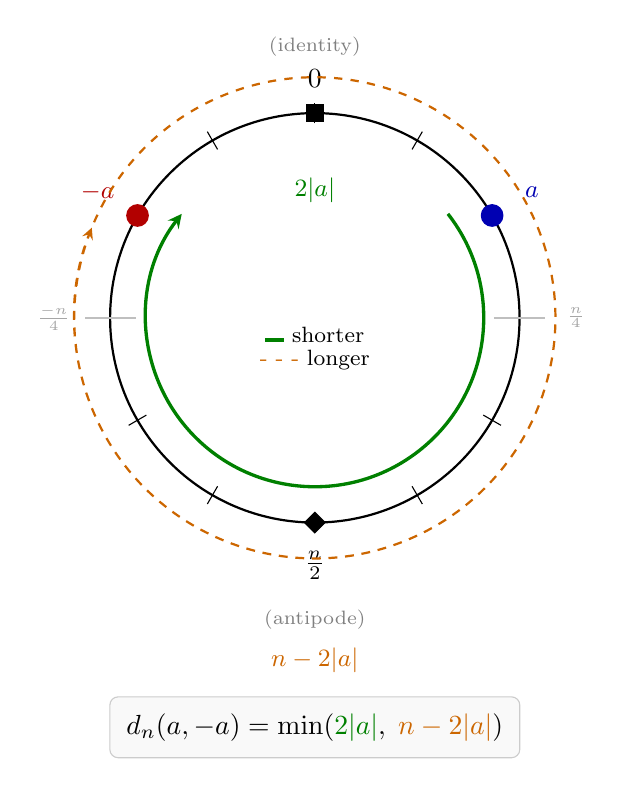
\begin{tikzpicture}[scale=1.3]
  % Draw main circle
  \draw[thick] (0,0) circle (2cm);

  % Draw tick marks for n=12
  \foreach \i in {0,...,11} {
    \draw ({90 - \i*30}:1.9) -- ({90 - \i*30}:2.1);
  }

  % Threshold markers at n/4 and -n/4 (positions 3 and 9 for n=12)
  \draw[gray!50, thick] ({90 - 3*30}:1.75) -- ({90 - 3*30}:2.25);
  \draw[gray!50, thick] ({90 - 9*30}:1.75) -- ({90 - 9*30}:2.25);
  \node[gray!70, font=\scriptsize] at ({90 - 3*30}:2.55) {$\frac{n}{4}$};
  \node[gray!70, font=\scriptsize] at ({90 - 9*30}:2.55) {$\frac{-n}{4}$};

  % Identity marker at 0 (filled square)
  \filldraw[black] (90:2) +(-0.08,-0.08) rectangle +(0.08,0.08);
  \node[above] at (90:2.15) {$0$};
  \node[gray, font=\scriptsize] at (90:2.65) {(identity)};

  % Antipode marker at n/2 (filled diamond)
  \filldraw[black] (-90:2) +(-0.1,0) -- +(0,0.1) -- +(0.1,0) -- +(0,-0.1) -- cycle;
  \node[below] at (-90:2.18) {$\frac{n}{2}$};
  \node[gray, font=\scriptsize] at (-90:2.95) {(antipode)};

  % Point a at position 2 (60 degrees from top, clockwise)
  \filldraw[blue!70!black] ({90 - 2*30}:2) circle (3pt);
  \node[blue!70!black, font=\small] at ({90 - 2*30}:2.45) {$a$};

  % Point -a at position 10 (symmetric)
  \filldraw[red!70!black] ({90 - 10*30}:2) circle (3pt);
  \node[red!70!black, font=\small] at ({90 - 10*30}:2.45) {$-a$};

  % Draw shorter arc (solid green, through 0)
  \draw[green!50!black, very thick, -stealth]
    ({90 - 2*30 + 8}:1.65) arc ({90 - 2*30 + 8}:{90 - 10*30 - 8}:1.65);
  % Label on the arc
  \node[green!50!black, font=\small] at (90:1.25) {$2|a|$};

  % Draw longer arc (dashed orange, through n/2)
  \draw[orange!80!black, thick, dashed, -stealth]
    ({90 - 2*30 - 8}:2.35) arc ({90 - 2*30 - 8}:{90 - 10*30 + 8 - 360}:2.35);
  % Label on the arc
  \node[orange!80!black, font=\small] at (-90:3.35) {$n - 2|a|$};

  % Legend inside the circle (centered)
  \node[align=center, font=\footnotesize] at (0, -0.3) {%
    \textcolor{green!50!black}{\rule{0.8em}{1.5pt}} shorter\\[-1pt]
    \textcolor{orange!80!black}{- - -} longer};

  % Formula box at bottom (integrated into figure)
  \node[draw=gray!40, rounded corners=3pt, fill=gray!5, inner sep=6pt]
    at (0, -4.0) {$d_n(a, -a) = \min(\textcolor{green!50!black}{2|a|},\; \textcolor{orange!80!black}{n - 2|a|})$};
\end{tikzpicture}
\caption{Circular distance on $\Z_n$. Point $a$ and its reflection $-a \equiv n - a$ are shown. The gray threshold markers at $\pm n/4$ indicate where the shorter arc switches: when $|a| \leq n/4$, the shorter arc passes through $0$ (identity); when $|a| > n/4$, it passes through $n/2$ (antipode).}
\label{fig:circular}
\end{figure}

\subsection{Product Structure}

\begin{definition}[Product Metric on Cyclic Products]
For $X = \Z_{n_1} \times \cdots \times \Z_{n_k}$ and $x, y \in X$, the \emph{product metric} is:
\[
d(x, y) = \sum_{i=1}^k d_{n_i}(x_i, y_i)
\]
When $X$ is obtained from $\Z_n$ via CRT, this is the $\ell^1$ distance on the product decomposition, not the circular distance $d_n$ on $\Z_n$.
\end{definition}

\begin{definition}[Coordinate Negation Action]
The group $G = \Z_2^k$ acts on $X$ by:
\[
(g_1, \ldots, g_k) \cdot (x_1, \ldots, x_k) = ((-1)^{g_1} x_1, \ldots, (-1)^{g_k} x_k)
\]
The \emph{simple reflections} (also called \emph{coordinate reflections}) $S = \{s_1, \ldots, s_k\}$ are the generators, where $s_i$ negates only coordinate $i$.
\end{definition}

\subsection{Fiber Products}

\begin{definition}[Fiber Product]
Given homomorphisms $f: A \to C$ and $g: B \to C$, the fiber product is
\[
A \times_C B = \{(a, b) \in A \times B : f(a) = g(b)\}
\]
\end{definition}

\begin{proposition}[CRT as Fiber Product]\label{prop:crt}
For $d = \gcd(m, n)$ with canonical projections $\pi_m: \Z_m \to \Z_d$ and $\pi_n: \Z_n \to \Z_d$:
\[
\Z_m \times_{\Z_d} \Z_n \cong \Z_{\mathrm{lcm}(m, n)}
\]
\end{proposition}

The general fiber product structure:
\[
\begin{tikzcd}[row sep=large, column sep=large]
\Z_{\mathrm{lcm}(m,n)} \arrow[r, "\bmod m"] \arrow[d, "\bmod n"'] & \Z_m \arrow[d, "\bmod d"] \\
\Z_n \arrow[r, "\bmod d"'] & \Z_d
\end{tikzcd}
\]
where $d = \gcd(m, n)$. The top-left corner is the \emph{pullback} of the two projections.

\section{The Additivity Theorem}

\begin{definition}[Cost Function]
For $g \in G$ and $x \in X$, define $c_g(x) = d(x, g \cdot x)$.
\end{definition}

\begin{theorem}[Cost Additivity]\label{thm:additive}
Let $g = s_{i_1} \cdots s_{i_r}$ be a product of distinct simple reflections. Then:
\[
c_g(x) = \sum_{j=1}^r c_{s_{i_j}}(x)
\]
\end{theorem}

\begin{proof}
The simple reflection $s_i$ affects only coordinate $i$:
\[
c_{s_i}(x) = d_{n_i}(x_i, -x_i)
\]
For composite $g$ negating coordinates $\{i_1, \ldots, i_r\}$:
\[
c_g(x) = \sum_{j=1}^k d_{n_j}(x_j, (g \cdot x)_j) = \sum_{j \in \{i_1, \ldots, i_r\}} d_{n_j}(x_j, -x_j) + \sum_{j \notin \{i_1, \ldots, i_r\}} 0
\]
The result follows.
\end{proof}

\begin{figure}[ht]
\centering
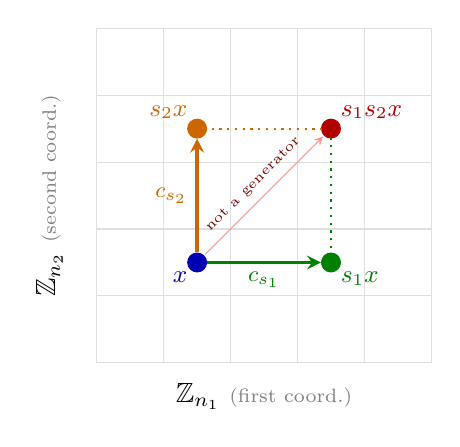
\begin{tikzpicture}[scale=0.85]
  % Grid representing Z_n1 x Z_n2 (smaller, centered)
  \def\cols{5}
  \def\rows{5}

  % Draw grid
  \foreach \x in {0,...,\cols} {
    \draw[gray!25] (\x, 0) -- (\x, \rows);
  }
  \foreach \y in {0,...,\rows} {
    \draw[gray!25] (0, \y) -- (\cols, \y);
  }

  % Axis labels
  \node at (2.5, -0.5) {$\Z_{n_1}$ \textcolor{gray}{\scriptsize (first coord.)}};
  \node[rotate=90] at (-0.7, 2.5) {$\Z_{n_2}$ \textcolor{gray}{\scriptsize (second coord.)}};

  % Point x at (1.5, 1.5)
  \filldraw[blue!70!black] (1.5, 1.5) circle (4pt);
  \node[blue!70!black, below left, font=\small] at (1.5, 1.5) {$x$};

  % s_1(x) at (3.5, 1.5) - horizontal reflection (GREEN)
  \filldraw[green!50!black] (3.5, 1.5) circle (4pt);
  \node[green!50!black, below right, font=\small] at (3.5, 1.5) {$s_1 x$};

  % s_2(x) at (1.5, 3.5) - vertical reflection (ORANGE)
  \filldraw[orange!80!black] (1.5, 3.5) circle (4pt);
  \node[orange!80!black, above left, font=\small] at (1.5, 3.5) {$s_2 x$};

  % s_1 s_2(x) at (3.5, 3.5) - composite (RED)
  \filldraw[red!70!black] (3.5, 3.5) circle (4pt);
  \node[red!70!black, above right, font=\small] at (3.5, 3.5) {$s_1 s_2 x$};

  % Arrow from x to s_1(x) - THICK GREEN with label
  \draw[-stealth, green!50!black, very thick] (1.65, 1.5) -- (3.35, 1.5);
  \node[green!50!black, below, font=\footnotesize] at (2.5, 1.5) {$c_{s_1}$};

  % Arrow from x to s_2(x) - THICK ORANGE with label
  \draw[-stealth, orange!80!black, very thick] (1.5, 1.65) -- (1.5, 3.35);
  \node[orange!80!black, left, font=\footnotesize] at (1.5, 2.5) {$c_{s_2}$};

  % Arrow from x to s_1 s_2(x) - THIN, LIGHT RED
  \draw[-stealth, red!40!white, thin] (1.62, 1.62) -- (3.38, 3.38);
  \node[red!50!black, font=\tiny, rotate=45, above] at (2.5, 2.5) {not a generator};

  % Manhattan path decomposition (colored to match)
  \draw[green!50!black, thick, dotted] (3.5, 1.6) -- (3.5, 3.4);
  \draw[orange!80!black, thick, dotted] (1.6, 3.5) -- (3.4, 3.5);
\end{tikzpicture}

\vspace{0.3em}
\[
\textcolor{red!70!black}{c_{s_1 s_2}(x)} \;=\; \textcolor{green!50!black}{c_{s_1}(x)} + \textcolor{orange!80!black}{c_{s_2}(x)}
\qquad\text{\small (no shortcut)}
\]

\vspace{-0.5em}
{\footnotesize
\textcolor{green!50!black}{\rule{1em}{2pt}} $s_1$: negates first coord.\quad
\textcolor{orange!80!black}{\rule{1em}{2pt}} $s_2$: negates second coord.\quad
\textcolor{red!40!white}{\rule{1em}{0.5pt}} $s_1 s_2$: composite%
}
\caption{Cost additivity on $\Z_{n_1} \times \Z_{n_2}$. Simple generators $s_1$ (green) and $s_2$ (orange) act on single coordinates. The composite $s_1 s_2$ (red diagonal) pays the full sum---dotted lines show the Manhattan decomposition.}
\label{fig:additivity}
\end{figure}

\begin{lemma}[The Core Inequality]\label{lem:core}
For any non-negative reals $a_1, \ldots, a_k$:
\[
\boxed{\min_i a_i \leq \sum_i a_i}
\]
In particular, for $k = 3$: $\min(a, b, c) \leq \min(a{+}b,\, a{+}c,\, b{+}c,\, a{+}b{+}c)$.
\end{lemma}

\noindent\textbf{All subsequent optimality results reduce to this inequality.}

\begin{proof}[Proof of Theorem~\ref{thm:main}]
By Theorem~\ref{thm:additive}, for any composite $h = s_{i_1} \cdots s_{i_r}$:
\[
c_h(x) = \sum_{j=1}^r c_{s_{i_j}}(x) \geq \min_{j} c_{s_{i_j}}(x) \geq \min_{s \in S} c_s(x)
\]
The first inequality is Lemma~\ref{lem:core}; the second is immediate.
\end{proof}

\begin{remark}[Universality]
Once distance is additive, composite reflections cannot produce emergent savings. The geometry admits no ``shortcuts''---every composite pays the full cost of each component. This is independent of the specific cycle sizes $n_i$. More precisely, the result depends on three properties: (1) additive metric decomposition, (2) involutive generators, and (3) disjoint supports---not on the arithmetic structure of $\Z_n$ per se.
\end{remark}

\begin{corollary}[Greedy Optimality]
The greedy rule ``pair $x$ with $s \cdot x$ where $s \in S$ minimizes $c_s(x)$'' defines an involution (by Proposition~\ref{prop:exist}) and achieves the global optimum among all orbit-respecting matchings.
\end{corollary}

\section{Application: Calendar Round}

The Calendar Round provides our first example of fiber product structure in a calendar system. The structural observations in this section (fiber decomposition, shared $\Z_5$ component, symmetry reduction) are independent of any metric. The optimality result (\S\ref{prop:cr-decomp}) applies to the product metric on the CRT decomposition.

\subsection{Fiber Product Structure}

\begin{proposition}\label{prop:cr-structure}
$\gcd(260, 365) = 5$ and $\mathrm{lcm}(260, 365) = 18980$.
\end{proposition}

\begin{proposition}\label{prop:cr-fiber}
The fiber product diagram
\[
\begin{tikzcd}
\Z_{18980} \arrow[r] \arrow[d] & \Z_{260} \arrow[d, "\bmod 5"] \\
\Z_{365} \arrow[r, "\bmod 5"'] & \Z_5
\end{tikzcd}
\]
is a pullback square.
\end{proposition}

\begin{proposition}[Shared Component]\label{prop:z5-shared}
For all $d \in \Z_{18980}$:
\[
(d \bmod 260) \bmod 5 = (d \bmod 365) \bmod 5 = d \bmod 5
\]
\end{proposition}

\begin{proof}
Since $5 \mid 260$ and $5 \mid 365$, both reductions factor through $d \bmod 5$.
\end{proof}

\subsection{Symmetry Group and Product-Metric Optimality}

\begin{proposition}\label{prop:cr-decomp}
$\Z_{18980} \cong \Z_4 \times \Z_5 \times \Z_{13} \times \Z_{73}$ (via CRT).
\end{proposition}

\begin{definition}[Fiber-Preserving Action]
The group $\Z_2^3$ acts on $(\Z_4, \Z_{13}, \Z_{73})$ by coordinate negation, fixing the $\Z_5$ factor.
\end{definition}

\begin{proof}[Proof of Corollary~\ref{cor:cr}]
By Theorem~\ref{thm:main} applied to $\Z_4 \times \Z_{13} \times \Z_{73}$ with the product metric and the restricted action.
\end{proof}

\begin{remark}
The constraint $5 \mid \gcd(260, 365)$ reduces the symmetry group from $\Z_2^4$ to $\Z_2^3$. This is a structural fact, independent of any metric.
\end{remark}

\section{Application: Sexagenary Cycle (\cjk{干支})}

The Chinese Sexagenary Cycle (\cjk{干支}, \emph{gānzhī}) combines ten Heavenly Stems (\cjk{天干}) with twelve Earthly Branches (\cjk{地支}) to form a 60-year cycle. As with the Calendar Round, the main observation is structural: the cycle is a fiber product with a culturally meaningful shared component.

\subsection{Fiber Product Structure}

\begin{proposition}\label{prop:sex-structure}
$\gcd(10, 12) = 2$ and $\mathrm{lcm}(10, 12) = 60$.
\end{proposition}

\begin{proposition}\label{prop:sex-fiber}
The fiber product diagram
\[
\begin{tikzcd}
\Z_{60} \arrow[r] \arrow[d] & \Z_{10} \arrow[d, "\bmod 2"] \\
\Z_{12} \arrow[r, "\bmod 2"'] & \Z_2
\end{tikzcd}
\]
is a pullback square.
\end{proposition}

\begin{proposition}[Shared Component]\label{prop:z2-shared}
For all $y \in \Z_{60}$:
\[
(y \bmod 10) \bmod 2 = (y \bmod 12) \bmod 2 = y \bmod 2
\]
\end{proposition}

\begin{proof}
Since $2 \mid 10$ and $2 \mid 12$, both reductions factor through $y \bmod 2$.
\end{proof}

\subsection{Symmetry Group and Product-Metric Optimality}

\begin{proposition}\label{prop:sex-decomp}
$\Z_{60} \cong \Z_5 \times \Z_4 \times \Z_3$ (via CRT), where $\Z_4 \supset \Z_2$.
\end{proposition}

\begin{definition}[Fiber-Preserving Action]
The group $\Z_2^2$ acts on $(\Z_5, \Z_3)$ by coordinate negation, fixing the $\Z_4$ factor.
\end{definition}

\begin{proof}[Proof of Corollary~\ref{cor:sex}]
By Theorem~\ref{thm:main} applied to $\Z_5 \times \Z_3$ with the product metric and the restricted action.
\end{proof}

\begin{remark}
The constraint $2 \mid \gcd(10, 12)$ reduces the symmetry group from $\Z_2^3$ to $\Z_2^2$. This is a structural fact, independent of any metric.
\end{remark}

\subsection{Parity Constraint}

\begin{corollary}[Parity Equality]\label{cor:parity}
Valid pairs $(s, b) \in \Z_{10} \times \Z_{12}$ representing elements of $\Z_{60}$ satisfy:
\[
s \bmod 2 = b \bmod 2
\]
\end{corollary}

\begin{remark}
In the traditional Chinese calendar, this parity corresponds to the yin/yang (\cjk{陰}/\cjk{陽}) classification: elements with $s \equiv 0 \pmod 2$ are ``yang'' (\cjk{陽}), those with $s \equiv 1 \pmod 2$ are ``yin'' (\cjk{陰}). The fiber product condition forces yang components to pair with yang, yin with yin.
\end{remark}

\section{Contrast: Boolean Hypercube}

Hamming distance is itself additive across coordinates:
\[
d_H(x, y) = \sum_{i=1}^n \mathbf{1}[x_i \neq y_i]
\]
However, the natural generators on $\{0,1\}^n$---complement and reversal---are \emph{not} coordinate-local.

\begin{definition}[Non-Local Generators]
On $\{0,1\}^6$:
\begin{itemize}
    \item Complement $c(h)_i = 1 - h_i$ flips \emph{all} coordinates
    \item Reversal $r(h)_i = h_{5-i}$ \emph{permutes} coordinates
\end{itemize}
Neither acts on a single coordinate while fixing others.
\end{definition}

\begin{figure}[ht]
\centering
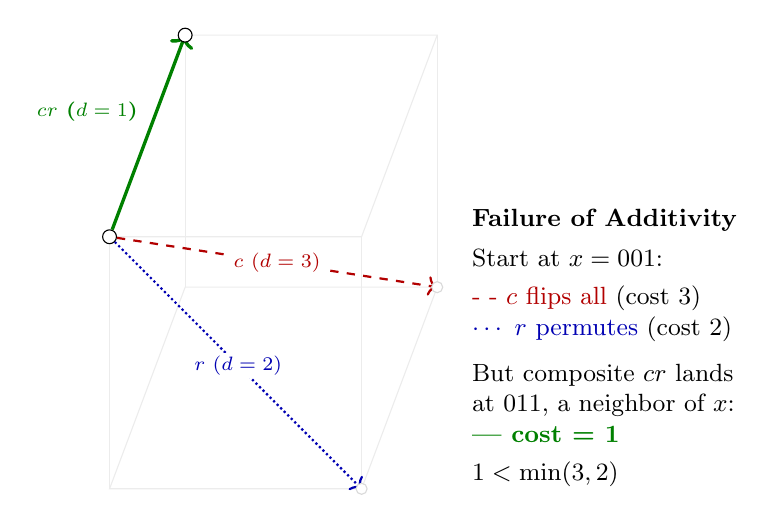
\begin{tikzpicture}[scale=1.6,
    vertex/.style={circle, draw=gray!30, fill=white, minimum size=4pt, inner sep=0pt},
    active/.style={circle, draw=black, fill=black, minimum size=5pt, inner sep=0pt},
    target/.style={circle, draw=black, fill=green!60!black, minimum size=5pt, inner sep=0pt},
    ghost/.style={gray!15, thin},
    label/.style={font=\scriptsize, fill=white, inner sep=1pt, text=black!80}
  ]
  % 3D cube configuration
  \def\d{2.0}  % size
  \def\p{0.6}  % perspective depth

  % -- 1. GHOST CUBE (Background context) --
  % Vertices
  \coordinate (000) at (0, 0);
  \coordinate (100) at (\d, 0);
  \coordinate (010) at (\p, \p+\d*0.5);
  \coordinate (110) at (\d+\p, \p+\d*0.5);
  \coordinate (001) at (0, \d);
  \coordinate (101) at (\d, \d);
  \coordinate (011) at (\p, \p+\d*1.5);
  \coordinate (111) at (\d+\p, \p+\d*1.5);

  % Edges (Ghosted)
  \draw[ghost] (000)--(100)--(110)--(010)--cycle;
  \draw[ghost] (001)--(101)--(111)--(011)--cycle;
  \draw[ghost] (000)--(001) (100)--(101) (010)--(011) (110)--(111);

  % -- 2. THE NARRATIVE (Active elements) --

  % START NODE: x = 001
  \node[active, label={left:\textbf{001} ($x$)}] (N001) at (001) {};

  % REVERSAL: r(x) = 100
  \draw[blue!70!black, thick, densely dotted, ->] (N001) -- (100)
    node[midway, label, text=blue!70!black] {$r$ ($d=2$)};
  \node[vertex, label={below right:100}] at (100) {};

  % COMPLEMENT: c(x) = 110
  \draw[red!70!black, thick, dashed, ->] (N001) -- (110)
    node[midway, label, text=red!70!black] {$c$ ($d=3$)};
  \node[vertex, label={right:110}] at (110) {};

  % COMPOSITE: cr(x) = 011 -- the shortcut!
  \draw[green!50!black, very thick, ->] (N001) -- (011)
    node[midway, above left, font=\scriptsize\bfseries, text=green!50!black] {$cr$ ($d=1$)};
  \node[target, label={above:011}] at (011) {};

  % -- 3. LEGEND / EXPLANATION --
  \node[anchor=north west, align=left, font=\small] at (\d+0.8, \d+0.3) {
    \textbf{Failure of Additivity}\\[0.4em]
    Start at $x=001$:\\[0.3em]
    \textcolor{red!70!black}{- - $c$ flips all} (cost 3)\\
    \textcolor{blue!70!black}{$\cdots$ $r$ permutes} (cost 2)\\[0.6em]
    But composite $cr$ lands\\
    at 011, a neighbor of $x$:\\
    \textcolor{green!50!black}{\textbf{--- cost = 1}}\\[0.3em]
    $1 < \min(3, 2)$
  };
\end{tikzpicture}
\caption{Non-locality on $\{0,1\}^3$. Simple generators $c$ (complement) and $r$ (reversal) send $x=001$ to distant vertices (distances 3 and 2), but the composite $cr$ lands on an immediate neighbor (distance 1). The geometry admits ``shortcuts'' via composition, violating cost additivity.}
\label{fig:hypercube}
\end{figure}

\begin{proposition}[Failure of Cost Additivity under Composition]\label{prop:hamming}
For the generators $c$ and $r$ on $\{0,1\}^6$, the identity
\[
d_H(h, c(r(h))) = d_H(h, c(h)) + d_H(h, r(h))
\]
fails in general. In fact, for hexagrams with $d_H(h, r(h)) = 4$:
\[
d_H(h, c(r(h))) = 2 < 4 = \min(d_H(h, c(h)), d_H(h, r(h)))
\]
\end{proposition}

\begin{proof}
Direct computation. When $r(h)$ differs from $h$ in exactly 4 positions, applying $c$ to $r(h)$ flips all bits, leaving only 2 positions different from $h$.
\end{proof}

\begin{theorem}[I Ching Requires Composites~\cite{radisic2026iching}]
The optimal $K_4$-equivariant matching on $\{0,1\}^6$ has total Hamming cost $96$. Any matching using only $c$ or $r$ pairings has cost at least $120$.
\end{theorem}

\begin{remark}
The contrast with cyclic products is now precise: in $\Z_{n_1} \times \cdots \times \Z_{n_k}$, each generator $s_i$ negates \emph{only} coordinate $i$, so generators have disjoint supports and cost is additive under composition. On $\{0,1\}^n$, the generators $c$ and $r$ have overlapping, non-local supports, so the additivity argument fails.
\end{remark}

\begin{remark}[Scope of the Theorem]
Theorem~\ref{thm:general} requires generators with \emph{disjoint supports}. It does not apply to:
\begin{itemize}
    \item Systems where generators act on multiple coordinates (e.g., complement on $\{0,1\}^n$).
    \item Non-additive metrics, even with coordinate-local generators.
    \item Groups not generated by commuting involutions.
\end{itemize}
The additivity of the metric alone is insufficient; what matters is that each generator affects exactly one summand.
\end{remark}

\section{The Dual Problem: Maximum Distance Matching}

The preceding sections concern \emph{minimization} of pairing distance. We now consider the dual: \emph{maximization}. This reversal admits a unique solution with a remarkably simple structure.

\subsection{Ifá Divination System}

The Yoruba Ifá tradition employs 256 figures called Odù, each consisting of two columns of four marks. Mathematically:

\begin{definition}[Odù]
An Odù is an element of $\{0,1\}^8$.
\end{definition}

The traditional pairings of Odù are by \emph{complement}: Ogbe (11111111) pairs with Oyeku (00000000), representing light and darkness; Iwori pairs with Odi, representing expansion and contraction.

\subsection{Complement as Unique Maximum}

\begin{theorem}[Maximum Distance Characterization]\label{thm:ifa-max}
For $x, y \in \{0,1\}^n$:
\[
d_H(x, y) = n \iff y = \bar{x}
\]
where $\bar{x}$ denotes the bitwise complement.
\end{theorem}

\begin{proof}
$d_H(x, \bar{x}) = n$ since every bit differs. Conversely, if $d_H(x, y) = n$, then $x_i \neq y_i$ for all $i$, so $y_i = 1 - x_i = \bar{x}_i$.
\end{proof}

\begin{corollary}[Unique Maximum Matching]\label{cor:ifa-unique}
The complement matching $\phi(x) = \bar{x}$ is the \emph{unique} matching on $\{0,1\}^n$ achieving maximum total Hamming distance.
\end{corollary}

\begin{proof}
Any matching achieving the maximum must have $d_H(x, \phi(x)) = n$ for all $x$. By Theorem~\ref{thm:ifa-max}, this forces $\phi(x) = \bar{x}$.
\end{proof}

\subsection{Duality with the I Ching}

\begin{center}
\begin{tabular}{lccl}
\toprule
\textbf{System} & \textbf{Space} & \textbf{Objective} & \textbf{Optimal Matching} \\
\midrule
I Ching & $\{0,1\}^6$ & Minimize & Composite ($c \circ r$) on some orbits \\
Ifá & $\{0,1\}^8$ & Maximize & Complement (unique) \\
\bottomrule
\end{tabular}
\end{center}

The contrast is instructive:
\begin{itemize}
    \item \textbf{Minimization} admits multiple local optima; the global optimum requires careful orbit-by-orbit analysis.
    \item \textbf{Maximization} admits a unique global optimum with trivial structure: complement every element.
\end{itemize}

\begin{remark}[Semantic Interpretation]
The duality reflects different pairing philosophies:
\begin{itemize}
    \item King Wen pairs by \emph{transformation}: hexagrams related by reversal or complement-reversal.
    \item Ifá pairs by \emph{opposition}: each Odù with its semantic opposite.
\end{itemize}
Both achieve optimality for their respective objectives.
\end{remark}

\section{Discussion}

\subsection{The Additivity Criterion}

The key distinction is not whether the \emph{metric} is additive (both Hamming and circular distance are), but whether the \emph{generators} are coordinate-local.

\begin{itemize}
    \item \textbf{Cyclic products}: Each generator $s_i$ negates only coordinate $i$. Generators have disjoint supports, so $c_{s_i s_j}(x) = c_{s_i}(x) + c_{s_j}(x)$.
    \item \textbf{Boolean hypercube}: Complement acts on all coordinates; reversal permutes them. Neither is local, so cost under composition is not additive.
\end{itemize}

This explains why composites can ``win'' in the I Ching: applying $c \circ r$ is not the same as paying $c$-cost plus $r$-cost.

\subsection{Fiber Constraints and Symmetry Reduction}

GCD constraints in calendar systems create fiber product structure, which \emph{locks} shared components. This reduces the available symmetry group. The locked component functions as a ``synchronization constraint'' between the two input cycles: any valid element must project consistently to both cycles modulo the GCD.

This structural observation is independent of any metric. Whether one measures distance by the native circular metric $d_n$, the product metric, or any other metric, the fiber decomposition and the resulting symmetry reduction remain the same.

\subsection{The CRT Isometry Gap}

The Chinese Remainder Theorem provides a group isomorphism $\Z_n \cong \Z_{n_1} \times \cdots \times \Z_{n_k}$, but this is \emph{not} an isometry between $(\Z_n, d_n)$ and $(\Z_{n_1} \times \cdots \times \Z_{n_k}, \sum_i d_{n_i})$. The product metric on the CRT decomposition is a different metric from the circular distance on $\Z_n$.

For example, in $\Z_{60} \cong \Z_5 \times \Z_4 \times \Z_3$:
\[
d_{60}(1, 2) = 1, \qquad d_5(1, 2) + d_4(1, 2) + d_3(1, 2) = 1 + 1 + 1 = 3
\]

Our optimality theorem (Theorem~\ref{thm:general}) applies to the product metric. Whether simple reflections are also optimal under the native circular metric $d_n$ is a separate question not addressed here. The structural results (fiber products, shared components, symmetry reduction) do not depend on the metric and hold unconditionally.

\subsection{Cross-Cultural Observations}

\emph{This subsection offers commentary on the cultural and historical context of the structural observations. These observations concern the fiber product decomposition, which is metric-independent. No claims of historical causation are made. Readers focused solely on the mathematics may skip to \S\ref{sec:verification}.}

\paragraph{Cross-Cultural Coincidence.}
The Calendar Round (Mesoamerican) and Sexagenary Cycle (Chinese) both exhibit fiber product structure, despite no documented contact between the civilizations. Both involve two input cycles with $\gcd > 1$, a shared component determined by the GCD, and resulting symmetry reduction.

From a mathematical perspective, this coincidence may be less surprising than it first appears: fiber product structure is \emph{nearly inevitable} when combining any two periodic systems $(\Z_m, \Z_n)$ that must remain synchronized on a common sub-cycle $\Z_{\gcd(m,n)}$. Any calendar designer seeking to track multiple astronomical periods (lunar months, solar years, ritual cycles) while maintaining internal consistency will naturally arrive at such a construction. The ``coincidence'' may thus reflect universal mathematical constraints on designing robust, interlocking calendars rather than cultural contact or pure chance.

\paragraph{Yin/Yang Correspondence.}
In the Sexagenary system, the $\Z_2$ fiber corresponds to the traditional yin/yang classification. The constraint of Corollary~\ref{cor:parity}---that valid pairs must have matching parity---is mathematically equivalent to the traditional rule that yang Heavenly Stems pair only with yang Earthly Branches. This equivalence is a structural fact about the fiber product, not a metric property. We make no claim about whether this correspondence was known to ancient practitioners; we note only the formal equivalence.

\section{Formal Verification}\label{sec:verification}

\paragraph{Lean 4 / Mathlib.}
The Lean formalization defines the product metric explicitly (as \texttt{sexDist} and \texttt{crDist}, the sum of circular distances on each CRT factor). The Sexagenary Cycle ($n = 60$) optimality is verified exhaustively via \texttt{native\_decide}. The Calendar Round ($n = 18980$) is proven structurally via cost additivity, requiring no enumeration. The key insight is that composite costs decompose as sums of simple costs under the product metric, reducing optimality to a pure arithmetic inequality ($\min(a,b,c) \leq \min(a{+}b, a{+}c, b{+}c, a{+}b{+}c)$) that \texttt{omega} discharges instantly. The fiber product structure, shared component theorems, and symmetry preservation lemmas are verified independently and do not depend on any metric.

\paragraph{Structural vs.\ Computational Proofs.}
The Calendar Round proof demonstrates a general principle: when generators have disjoint supports, cost additivity enables \emph{structural} proofs that scale independently of $n$. This contrasts with brute-force enumeration, which becomes infeasible for large $n$.

\begin{center}
\begin{tabular}{lllc}
\toprule
\textbf{Theorem} & \textbf{File} & \textbf{Method} & \textbf{Kernel-Checked} \\
\midrule
\texttt{cost\_additive} & \texttt{Sexagenary/Optimality} & \texttt{native\_decide} & \checkmark \\
\texttt{simple\_always\_optimal} & \texttt{Sexagenary/Optimality} & \texttt{native\_decide} & \checkmark \\
\texttt{z2\_shared} & \texttt{Sexagenary/Basic} & \texttt{omega} & \checkmark \\
\texttt{z5\_shared} & \texttt{CalendarRound/Basic} & \texttt{omega} & \checkmark \\
\texttt{simple\_always\_optimal} & \texttt{CalendarRound/Optimality} & proof + \texttt{omega} & \checkmark \\
\texttt{hammingDist\_complement} & \texttt{Ifa/Odu} & proof & \checkmark \\
\texttt{complement\_uniquely\_maximum} & \texttt{Ifa/Optimality} & proof & \checkmark \\
\bottomrule
\end{tabular}
\end{center}

\paragraph{Code Availability.}
Lean 4 source code is available at \url{https://github.com/alerad/calendars}.

\section{Conclusion}

We have identified two contributions of independent interest:

\paragraph{Structural.} The Mesoamerican Calendar Round and Chinese Sexagenary Cycle both decompose as fiber products of their constituent cycles, with shared components ($\Z_5$ and $\Z_2$ respectively) that constrain the symmetry group. These fiber product structures arise independently in unconnected civilizations and correspond to culturally recognized features. The structural observation is metric-independent.

\paragraph{Optimality.} For any product of cyclic groups with the product metric (sum of circular distances on each factor), simple coordinate reflections always achieve optimal pairing cost. The proof reduces to cost additivity under generator composition plus a trivial arithmetic inequality. This theorem applies to the CRT decomposition of the calendar systems, but not to the native circular metric $d_n$, since the CRT is not an isometry. The contrast with the Boolean hypercube clarifies the precise criterion: the locality of generators, not the metric alone, determines whether composite operations can outperform simple ones.

The dual problem (maximization rather than minimization) admits a unique and trivial solution: complement pairing. The Yoruba Ifá tradition realizes this optimum, providing a cross-cultural counterpoint to the I Ching's minimization structure.

\begin{thebibliography}{9}

\bibitem{radisic2026iching}
Alejandro Radisic.
\newblock Optimal Equivariant Matchings on the 6-Cube: With an Application to the King Wen Sequence.
\newblock \emph{arXiv preprint} arXiv:2601.07175, 2026.
\newblock \url{https://arxiv.org/abs/2601.07175}

\bibitem{maclane1971}
Saunders Mac Lane.
\newblock {\em Categories for the Working Mathematician}.
\newblock Springer-Verlag, 1971.

\bibitem{bascom1969}
William Bascom.
\newblock {\em Ifa Divination: Communication Between Gods and Men in West Africa}.
\newblock Indiana University Press, 1969.

\end{thebibliography}

\end{document}
